\documentclass[10pt,openany]{book}
\usepackage{ctex} 
\usepackage{geometry,graphicx,xcolor,color}
\geometry{
	a4paper,
	top=25.4mm, bottom=25.4mm,
	left=20mm, right=20mm,
	headheight=2.17cm,
	headsep=4mm,
	footskip=12mm
}

\usepackage{amssymb,amsmath,mathrsfs}                    % 数学字体
\usepackage{mathpazo}% 采用 Palatino 风格字体
\usepackage[nofontspec]{newpxtext}

\definecolor{winered}{rgb}{0.5,0,0}
\definecolor{structurecolor}{RGB}{122,122,142}
\definecolor{main}{HTML}{3D445F}
\definecolor{second}{HTML}{627581}
\definecolor{third}{HTML}{9D8798}

% 定义引用的颜色
\usepackage{hyperref}
\hypersetup{colorlinks = true, linktoc=all, linkcolor=black, urlcolor=winered}

% ------------------------------------------------------------%
% 定义定理环境
\usepackage{amsthm}
\newtheoremstyle{defstyle}{3pt}{3pt}{\kaishu}{-3pt}{\bfseries\color{main}}{}{0.5em}{\indent 【\thmname{#1} \thmnumber{#2}】 \thmnote{(#3)}}
\newtheoremstyle{thmstyle}{3pt}{3pt}{\kaishu}{-3pt}{\bfseries\color{second}}{}{0.5em}{\indent【\thmname{#1} \thmnumber{#2}】 \thmnote{(#3)}}
\newtheoremstyle{prostyle}{3pt}{3pt}{\kaishu}{-3pt}{\bfseries\color{third}}{}{0.5em}{\indent【\thmname{#1} \thmnumber{#2}】 \thmnote{(#3)}}

\theoremstyle{thmstyle} %theorem style
\newtheorem{theorem}{定理}[chapter]
\theoremstyle{defstyle} % definition style
\newtheorem{definition}[theorem]{定义}
\newtheorem{lemma}[theorem]{引理}
\newtheorem{corollary}[theorem]{推论}
\theoremstyle{prostyle} % proposition style
\newtheorem{proposition}[theorem]{命题}
\newtheorem{example}[theorem]{例题}
\newtheorem{remark}[theorem]{注}

\renewenvironment{proof}[1][证明]{\par\underline{\textbf{#1.}} \;\fangsong}{\qed\par}
\newenvironment{solution}{\par\underline{\textbf{解.}} \;\kaishu}{\qed\par}
\newcommand{\intro}[1]{\rightline{\parbox[t]{5cm}{\footnotesize \fangsong\quad\quad #1 }}}
% ------------------------------------------------------------%
% ------------------------------------------------------------%
% 设置章节形式

\usepackage{titlesec, titletoc}
\linespread{1.2} 				
\usepackage{fancyhdr}
\fancyhf{}
\renewcommand{\headrule}{\color{structurecolor}\hrule width\textwidth}
\pagestyle{fancy}
\renewcommand{\headrulewidth}{1pt}
\fancypagestyle{plain}{
	\renewcommand{\headrulewidth}{0pt}
	\fancyhf{}
	\fancyfoot[c]{\color{structurecolor}\small\thepage}
	\renewcommand{\headrule}{}
	}

\fancyhead[c]{\color{structurecolor}\kaishu\rightmark}
\fancyfoot[c]{\color{structurecolor}\small\thepage}

\titleformat{\chapter}[display]{\Large}
{\color{structurecolor}\filleft
	\parbox{1cm}{\vbox to 1.5cm{\vfill\hbox to 4cm{\hfill\Huge \bfseries \color{structurecolor}{Chapter} \thechapter \hfill}}}}
{1ex}
{\color{structurecolor} \titlerule[2pt]\large\bfseries \filright \vspace*{1em}}
[\vspace*{1em} {\titlerule[2pt]}]

\titleformat{\section}[frame]{\normalfont\color{structurecolor}}{\footnotesize \enspace \large \textcolor{structurecolor}{\S \,\thesection}\enspace}{6pt}{\Large\filcenter \bf \kaishu }


\titleformat{\subsection}[hang]{\bfseries}{\large\bfseries\color{structurecolor}\thesubsection\enspace}{1pt}{\color{structurecolor}\large\bfseries\filright}

\titleformat{\subsubsection}[hang]{\bfseries}{\large\bfseries\color{structurecolor}\thesubsubsection\enspace}{1pt}{\color{structurecolor}\large\bfseries\filright}

% ------------------------------------------------------------%
% 设置封面
\usepackage{titling}
\renewcommand*{\maketitle}{
	\begin{titlepage}
		\newgeometry{margin = 0in}
		\parindent=0pt
		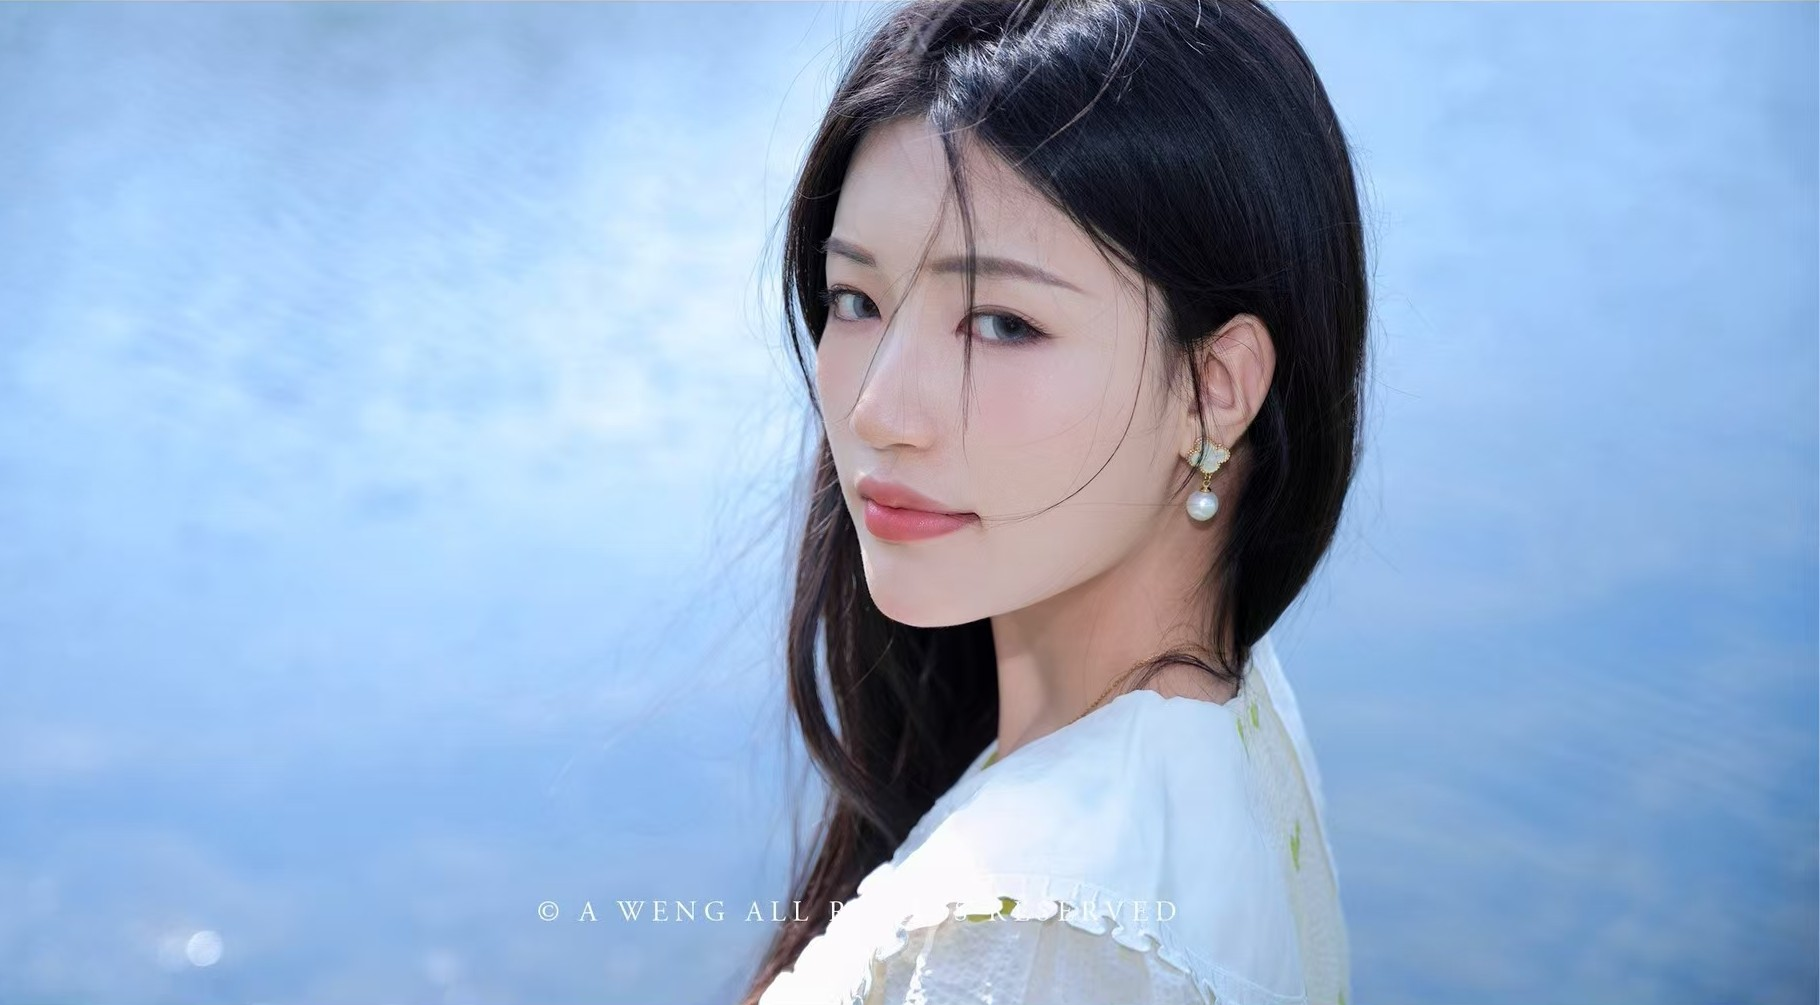
\includegraphics[scale=0.44]{Pictures/Cover_images/7_2.jpg}
		\vfill
		\begin{center}
			\parbox{0.618\textwidth}{
				\hfill {\bfseries \Huge \thetitle} \\[0.6pt]  
				\rule{0.618\textwidth}{4pt} \\ 
			}
		\end{center}
		\vfill
		\begin{center}
			\parbox{0.618\textwidth}{
				\hfill\Large
				\kaishu 
				\begin{tabular}{r|}
					作者:\theauthor \\ 
					时间:\thedate \\
				\end{tabular}
			}
		\end{center}
		\vfill
		\begin{center}
			\parbox[t]{0.7\textwidth}{\centering \kaishu }
		\end{center}
		\vfill
	\end{titlepage}
	\restoregeometry
	\thispagestyle{empty}
}
% ------------------------------------------------------------%

\title{学习笔记}
% \author{\href{https://www.zhihu.com/people/moment-jue-wang-30}{北斗逍遥-张嘉}}
\author{北斗逍遥-张嘉}
\date{\today}

% ------------------------------------------------------------%

% 参考文献配置
\bibliographystyle{plain}

% ------------------------------------------------------------%
% 代码块的配置
\usepackage{listings}  % 代码块宏包
\usepackage{xcolor}    % 颜色支持

% 配置 listings
\lstset{
	language=Python,       % 默认语言(可在环境里覆盖)
	frame=shadowbox,       % 边框样式:shadowbox(阴影框)/ single(实线框)/ double(双线框)
	rulesepcolor=\color{gray},  % 边框颜色
	backgroundcolor=\color{gray!5},  % 代码块背景色(浅灰色)
	tabsize=4,	% 缩进长度
	numbers=left,          % 显示行号
	numberstyle=\tiny\color{gray},  % 行号样式
	keywordstyle=\color{blue},      % 关键字颜色
	commentstyle=\color{green!60!black},  % 注释颜色
	stringstyle=\color{red},        % 字符串颜色
	basicstyle=\ttfamily\small,    % 代码字体(等宽+小字号)
	breaklines=true,                % 自动换行
	captionpos=b,                  % 标题位置(b=底部,t=顶部)
}

% ------------------------------------------------------------%
% 常用配置
\usepackage{comment}
\usepackage{tikz}
\usetikzlibrary{3d,calc,intersections}
\usepackage{float}
\usepackage{subcaption}
\usepackage{tikz-3dplot} %%三维图形绘制需要的宏包
\usetikzlibrary{patterns}%%填充使用的宏包




% ------------------------------------------------------------%
\begin{document}
\frontmatter

\maketitle

\tableofcontents

\mainmatter

% ------------------------------------------------------------%
% 置放章节
\chapter{第一章:数学工具篇}

\section{分析篇}

















































\section{代数篇}

\section{概率论与数理统计篇}
% ------------------------------------------------------------------------------------------- %
\subsection{基础知识}



% ------------------------------------------------------------------------------------------- %
\subsection{随机过程}


% ------------------------------------------------------------------------------------------- %
\subsection{马尔可夫相关}





% ------------------------------------------------------------------------------------------- %




\section{数论篇}

\section{实变函数篇}

\section{泛函分析篇}

\section{常微分方程篇}

\section{拓扑篇}









\newpage
\chapter{第二章:理论分析证明框架汇总}

\section{零阶优化算法}

% ------------------------------------------------------------------------------------------ %
\subsection{相关概念}


% ------------------------------------------------------------------------------------------ %
\subsection{常见的假设}








% ------------------------------------------------------------------------------------------ %
\subsection{收敛性分析}




% ------------------------------------------------------------------------------------------ %





\section{内存分析}

% \section{内存分析}

% \section{内存分析}

% \section{内存分析}

% \section{内存分析}

% \section{内存分析}



















\newpage
\chapter{第三章:AI 代码整理}

\section{Pytorch 辅助性工具}

% --------------------------------------------------------------------------------------------- %
% --------------------------------------------------------------------------------------------- %
\subsection{日志管理}
在软件开发、系统运维等领域,logging 日志是一种非常重要的记录机制,其核心作用是追踪系统运行过程中的关键信息、行为和状态,以便于后续的调试、监控、分析和问题排查。
% --------------------------------------------------------------------------------------------- %
\subsubsection{基本日志配置}
基本示例如下:
\begin{lstlisting}[language=python,caption={基本日志配置},label=code:log_configuration]
	import logging
	import os
	from datetime import datetime
	
	def setup_logger(log_dir="logs"):
		# 创建日志目录
		if not os.path.exists(log_dir):
		os.makedirs(log_dir)
	
		# 日志文件名:包含时间戳
		timestamp = datetime.now().strftime("%Y%m%d_%H%M%S")
		log_file = os.path.join(log_dir, f"training_{timestamp}.log")
	
		# 配置日志
		logging.basicConfig(
		level=logging.INFO,  # 日志级别:DEBUG, INFO, WARNING, ERROR, CRITICAL
		format="%(asctime)s-%(name)s-%(levelname)s-%(message)s",
		handlers=[
		logging.FileHandler(log_file),  # 输出到文件
		logging.StreamHandler()         # 同时输出到控制台
		]
		)
	
		return logging.getLogger(__name__)
	
	# 使用示例
	logger = setup_logger()
	logger.debug("这是调试信息")    # 不会显示,因为级别是INFO
	logger.info("训练开始")        # 会显示
	logger.warning("学习率可能过高")
	logger.error("数据加载失败")
\end{lstlisting}


% --------------------------------------------------------------------------------------------- %
\subsubsection{日志文件管理}
基本示例如下:
\begin{lstlisting}[language=python,caption={日志文件的轮转},label=code:Log_File_Management]
	import logging
	from logging.handlers import RotatingFileHandler, TimedRotatingFileHandler
	import os
	
	def setup_advanced_logger(log_dir="logs"):
		if not os.path.exists(log_dir):
		os.makedirs(log_dir)
	
		logger = logging.getLogger(__name__)
		logger.setLevel(logging.INFO)
	
		# 格式设置
		formatter = logging.Formatter("%(asctime)s-%(name)s-%(levelname)s-%(message)s")
	
		# 按大小轮转:每个文件最大10MB,保留5个备份
		file_handler = RotatingFileHandler(
		os.path.join(log_dir, "training.log"),
		maxBytes=10*1024*1024,  # 10MB
		backupCount=5,
		encoding="utf-8"
		)
	
		# 或者按时间轮转:每天一个日志文件
		# file_handler = TimedRotatingFileHandler(
		#     os.path.join(log_dir, "training.log"),
		#     when="D",  # 每天轮转
		#     interval=1,
		#     backupCount=7,  # 保留7天
		#     encoding="utf-8"
		# )
	
		file_handler.setFormatter(formatter)
		logger.addHandler(file_handler)
	
		# 同时输出到控制台
		console_handler = logging.StreamHandler()
		console_handler.setFormatter(formatter)
		logger.addHandler(console_handler)
	
		return logger
	
	# 在PyTorch训练中的使用示例
	def train_model(logger):
	logger.info("开始模型训练")
	for epoch in range(10):
	logger.info(f"=====第{epoch+1}轮训练=====")
	# 训练代码...
	loss = 0.5 - epoch*0.05  # 示例损失值
	accuracy = 0.6 + epoch*0.03  # 示例准确率
	logger.info(f"损失:{loss:.4f},准确率:{accuracy:.4f}")
	
	if loss < 0.2:
	logger.warning("损失值过低,可能存在过拟合风险")
	
	logger.info("模型训练完成")
\end{lstlisting}


% --------------------------------------------------------------------------------------------- %
\subsubsection{查看和解析日志文件}
基本示例如下:
\begin{lstlisting}[language=python,caption={解析日志文件},label=code:View_and_parse_logs]
	import re
	import pandas as pd
	
	def parse_log_file(log_path):
		"""解析日志文件,提取训练指标"""
		# 正则表达式匹配训练指标行
		pattern = r"(\d{4}-\d{2}-\d{2}\d{2}:\d{2}:\d{2})-.*-INFO-损失:([\d.]+),准确率:([\d.]+)"
	
		data = []
		with open(log_path, "r", encoding="utf-8") as f:
		for line in f:
			match = re.match(pattern, line.strip())
			if match:
				timestamp = match.group(1)
				loss = float(match.group(2))
				accuracy = float(match.group(3))
			data.append({
				"timestamp": timestamp,
				"loss": loss,
				"accuracy": accuracy
			})
	
		return pd.DataFrame(data)
	
	# 使用示例
	# df = parse_log_file("logs/training.log")
	# print(df)
\end{lstlisting}




% --------------------------------------------------------------------------------------------- %
\subsubsection{将日志信息整理到表格}
基本示例如下:
\begin{lstlisting}[language=python,caption={输出至表格},label=code:To_table]
	import pandas as pd
	import matplotlib.pyplot as plt
	
	def log_to_dataframe_and_visualize(log_path):
		# 解析日志文件
		df = parse_log_file(log_path)
	
		if df.empty:
		print("没有找到有效的训练指标数据")
		return
	
	# 保存为CSV文件
	df.to_csv("training_metrics.csv", index=False)
	print("训练指标已保存到 training_metrics.csv")
	
	# 可视化
	plt.figure(figsize=(12, 5))
	
	plt.subplot(1, 2, 1)
	plt.plot(df["loss"])
	plt.title("训练损失")
	plt.xlabel("轮次")
	plt.ylabel("损失值")
	
	plt.subplot(1, 2, 2)
	plt.plot(df["accuracy"])
	plt.title("训练准确率")
	plt.xlabel("轮次")
	plt.ylabel("准确率")
	
	plt.tight_layout()
	plt.savefig("training_metrics.png")
	plt.show()
	
	return df
	
	# 使用示例
	# metrics_df = log_to_dataframe_and_visualize("logs/training.log")
\end{lstlisting}

% --------------------------------------------------------------------------------------------- %
% --------------------------------------------------------------------------------------------- %
\subsection{终端自动化调参}
在深度学习(尤其是 PyTorch 训练)和日常开发中,shell 脚本(.sh 文件)是一种极其实用的工具,它的核心作用是自动化重复操作、批量执行命令、管理复杂工作流。
% --------------------------------------------------------------------------------------------- %
\subsubsection{shell-基础语法}
一些常见的语法可供查阅

\paragraph{声明变量}
\begin{lstlisting}[language=sh,caption={声明变量},label=code:shell_base1]
	# 声明一个变量
	name="John"
	# 声明变量并设置默认值
	name=${name:-zj}
	# 使用变量
	echo "Hello, $name!"  # 输出: Hello, John!
\end{lstlisting}


\paragraph{if-else}
\begin{lstlisting}[language=sh,caption={if-else语法},label=code:shell_base2]
	age=20
	# -eq:等于,--ne:不等于,-gt:大于,-lt:小于,-ge:大于等于,-le:小于等于
	if [ $age -ge 18 ]; then
	echo "You are an adult."
	elif
	echo "You are a minor."
	else
	echo "NO."
	fi	
\end{lstlisting}

\paragraph{case嵌套}
\begin{lstlisting}[language=sh,caption={case嵌套循环示例代码},label=code:shell_base3]
	case $TASK in
		CB)
			DEV=100
			;;
		Copa)
			DEV=100
			TASK_ARGS="--train_as_classification False"
			;;
		MultiRC)
			GA=$(expr $BS / 2)
			BS=2
			TASK_ARGS="--gradient_accumulation_steps $GA"
			;;
		ReCoRD)
			GA=$(expr $BS / 2)
			BS=2
			TASK_ARGS="--gradient_accumulation_steps $GA --train_as_classification False"
			;;
		*)
			# 默认处理
			;;
	esac
\end{lstlisting}

\paragraph{for循环}
\begin{lstlisting}[language=sh,caption={for-循环语法},label=code:shell_base4]
	# 输出 1 到 5 的数字
	for i in {1..5}; do
		echo "Number $i"
	done
\end{lstlisting}


\paragraph{while循环}
\begin{lstlisting}[language=sh,caption={while-循环语法},label=code:shell_base5]
	# 输出 1 到 5 的数字
	i=1
	while [ $i -le 5 ]; do
		echo "Number $i"
		i=$((i + 1))
	done
\end{lstlisting}


\paragraph{until循环}
\begin{lstlisting}[language=sh,caption={until-循环语法},label=code:shell_base6]
	# 输出 1 到 5 的数字
	i=1
	until [ $i -gt 5 ]; do
		echo "Number $i"
		i=$((i + 1))
	done
\end{lstlisting}


\paragraph{函数语法}
\begin{lstlisting}[language=sh,caption={函数},label=code:shell_base7]
	# 定义函数
	greet() {
		echo "Hello, $1!"
	}
	# 调用函数
	greet "Alice"  # 输出: Hello, Alice!
\end{lstlisting}


\paragraph{文件操作}
\begin{lstlisting}[language=sh,caption={文件操作},label=code:shell_base8]
	touch myfile.txt  # 创建一个空文件
	echo "This is a test." > myfile.txt  # 覆盖写入
	echo "Another line." >> myfile.txt  # 追加写入
	cat myfile.txt  # 显示文件内容
	rm myfile.txt  # 删除文件
	...
\end{lstlisting}

\subsubsection{shell-参数自动化调整}

\paragraph{自动化调参python-part}
\begin{lstlisting}[language=python,caption={调参},label=code:shell_tuning_py]
	import argparse
	from transformers import Trainer, TrainingArguments
	
	# 定义训练参数类
	@dataclass
	class OurArguments(TrainingArguments):
		task_name: str = "SST2"
		num_train: int = 0
		model_name: str = "facebook/opt-125m"
		# 其他参数...
	
	def parse_args():
		parser = argparse.ArgumentParser(description="Training script.")
		# 添加你的参数
		parser.add_argument("--task_name", type=str, default="SST2", help="Task name")
		parser.add_argument("--num_train", type=int, default=0, help="Number of training samples")
		parser.add_argument("--model_name", type=str, default="facebook/opt-125m", help="Model name")
		# 可以继续添加其他参数
		return parser.parse_args()
	
	def main():
		# 解析命令行参数
		args = parse_args()
	
	if __name__ == "__main__":
	main()
\end{lstlisting}


\paragraph{自动化调参shell-part}
\begin{lstlisting}[language=sh,caption={调参},label=code:shell_tuning_sh]
	#!/bin/bash
	
	# 定义任务、模型和训练样本数量的不同配置
	TASKS=("SST2" "RTE" "CB")
	MODEL_NAMES=("facebook/opt-125m" "google/bert-large-uncased")
	NUM_TRAIN_VALUES=(100 200 300)
	
	# 自动化调参
	for TASK in "${TASKS[@]}"
	do
		for MODEL in "${MODEL_NAMES[@]}"
		do
			for NUM_TRAIN in "${NUM_TRAIN_VALUES[@]}"
			do
				echo "Running for Task: $TASK, Model: $MODEL, Num_train: $NUM_TRAIN"
	
				# 执行 Python 脚本并传递参数
				python train.py --task_name $TASK --model_name $MODEL --num_train $NUM_TRAIN
			done
		done
	done
\end{lstlisting}

% --------------------------------------------------------------------------------------------- %
% --------------------------------------------------------------------------------------------- %
\subsection{进度条设置}
进度条需要采用tqdm包,基本使用方法如下:
\paragraph{基本用法}
\begin{lstlisting}[language=python,caption={示例},label=code:tqdb]
	from tqdm import tqdm
	import time
	
	## 1.基本用法
	# 普通循环(没有进度条)
	# for i in range(100):
	#     time.sleep(0.05)  # 模拟耗时操作
	
	# 用 tqdm 包装后(有进度条)
	for i in tqdm(range(100), desc="Processing", unit="单位"):
		time.sleep(0.05)  # 模拟耗时操作
		
	## 2.包装列表等可迭代对象
	items = ["a", "b", "c", "d", "e"] * 20  # 构造一个列表
	
	# 包装列表
	for item in tqdm(items, desc="Processing items"):
		time.sleep(0.1)  # 模拟处理每个元素的耗时
	
	## 3.手动更新进度条
	# 创建进度条对象,总步数为 3
	pbar = tqdm(total=3, desc="手动更新")
	# 第一步
	time.sleep(1)
	pbar.update(1)  # 进度 +1
	# 第二步
	time.sleep(1)
	pbar.update(1)  # 进度 +1
	# 第三步
	time.sleep(1)
	pbar.update(1)  # 进度 +1
	pbar.close()  # 关闭进度条
	
	## 4.在嵌套循环中使用
	epochs = 3  # 总轮次
	batchs_per_epoch = 10  # 每轮的批次
	
	# 外层循环:总训练进度
	global_pbar = tqdm(total=epochs * batchs_per_epoch, desc="总进度")
	
	for epoch in range(epochs):
		# 内层循环:当前epoch的进度(leave=False 表示完成后清除)
		epoch_pbar = tqdm(range(batchs_per_epoch), 
		desc=f"第 {epoch+1} 轮", 
		leave=False)
	
		for batch in epoch_pbar:
			time.sleep(0.2)  # 模拟训练一个批次
			global_pbar.update(1)  # 总进度 +1
			epoch_pbar.set_postfix(loss=0.5 - epoch*0.1)  # 显示额外信息(如损失)
		
		epoch_pbar.close()
		
	global_pbar.close()
\end{lstlisting}

% --------------------------------------------------------------------------------------------- %
% --------------------------------------------------------------------------------------------- %
\subsection{查询服务器显卡属性设置}

\paragraph{训练显存消耗记录}
\begin{lstlisting}[language=python,caption={查询显存},label=code:train_memory]
	import torch
	
	def track_gpu_memory(step_name):
		# 当前已分配显存
		current = torch.cuda.memory_allocated() / 1024**3
		# 历史最大显存(峰值)
		peak = torch.cuda.max_memory_allocated() / 1024**3
		# 重置峰值统计(可选,用于分阶段监控)
		# torch.cuda.reset_peak_memory_stats()
		print(f"[{step_name}] 显存: 当前 {current:.2f}GB | 峰值 {peak:.2f}GB")
	
	# 训练循环中关键节点调用
	for epoch in range(epochs):
		for inputs, labels in dataloader:
			# 前向传播前
			track_gpu_memory("前向传播前")
			
			# 前向传播
			outputs = model(inputs)
			loss = criterion(outputs, labels)
			track_gpu_memory("前向传播后")
			
			# 反向传播
			optimizer.zero_grad()
			loss.backward()
			track_gpu_memory("反向传播后")
			
			# 优化器更新
			optimizer.step()
			track_gpu_memory("优化器更新后")
			
			# 清空当前批次变量
			del inputs, labels, outputs, loss
			torch.cuda.empty_cache()  # 手动触发缓存清理(可选)
			track_gpu_memory("批次结束后")
\end{lstlisting}

\paragraph{训练时长消耗记录}
\begin{lstlisting}[language=python,caption={训练时长记录},label=code:train_time]
	import time
	from datetime import timedelta
	
	# 记录开始时间
	start_time = time.time()
	
	# 训练代码...
	for epoch in range(epochs):
		# 训练过程
		pass
	
	# 计算总时长
	total_time = time.time() - start_time
	print(f"总运行时间: {timedelta(seconds=int(total_time))}")
\end{lstlisting}

% --------------------------------------------------------------------------------------------- %
% --------------------------------------------------------------------------------------------- %
\subsection{wandb学习}
演示示例如下:
\begin{lstlisting}[language=python,caption={wandb记录},label=code:wandb]
	import wandb
	import random
	import numpy as np
	import os
	
	def main():
		# 1. wandb登录过程
		print("===== 登录到Weights & Biases =====")
		try:
			# 尝试检查登录状态
			api = wandb.Api()
			print("已登录到wandb")
		except Exception:
			print("未检测到登录状态,需要进行登录")
			# 优先从环境变量获取API密钥(适合服务器环境)
			api_key = os.getenv("WANDB_API_KEY")
			if api_key:
				wandb.login(key=api_key)
				print("通过环境变量成功登录")
			else:
				# 交互式登录(适合本地开发)
				print("请在弹出的浏览器中登录,或输入API密钥")
				wandb.login()
		
		# 2. 初始化wandb实验
		print("\n===== 初始化实验 =====")
			run = wandb.init(
			project="wandb-complete-demo",  # 项目名称
			name=f"demo-run-{random.randint(1000, 9999)}",  # 实验名称,包含随机数避免重复
			notes="这是一个wandb完整功能演示",  # 实验备注
			tags=["demo", "tutorial"],  # 实验标签
			config={  # 超参数配置
				"learning_rate": 0.01,
				"epochs": 20,
				"batch_size": 32,
				"optimizer": "Adam",
				"dataset": "synthetic"
			}
		)
		
		# 获取配置
		config = wandb.config
		
		# 3. 模拟训练数据
		print("\n===== 开始训练 =====")
		# 生成模拟数据分布的参数
		true_mean = 0.5
		true_std = 0.2
		
		# 4. 训练循环
		for epoch in range(config.epochs):
			# 模拟训练过程中的指标
			# 随着epoch增加,损失应该下降,准确率应该上升
			loss = (true_mean + np.random.normal(0, true_std)) / (epoch + 1)
			accuracy = 0.5 + (epoch / config.epochs) * 0.4 + np.random.normal(0, 0.03)
			accuracy = min(accuracy, 0.98)  # 限制最大准确率
			
			# 记录指标到wandb
			wandb.log({
				"training/loss": loss,
				"training/accuracy": accuracy,
				"training/epoch": epoch,
				# 可以记录更多衍生指标
				"training/loss_derivative": loss * 0.1 if epoch > 0 else 0
			})
			
			# 打印进度
			if epoch % 5 == 0:  # 每5个epoch打印一次
				print(f"Epoch {epoch:2d}/{config.epochs}: "
					f"Loss = {loss:.4f}, "
					f"Accuracy = {accuracy:.4f}")
		
		# 5. 完成实验
		print("\n===== 训练完成 =====")
		wandb.finish()
		print(f"实验已成功记录,可在以下地址查看:")
		print(f"https://wandb.ai/{wandb.run.entity}/{config.project}/runs/{wandb.run.id}")
	
	if __name__ == "__main__":
	main()
\end{lstlisting}



% --------------------------------------------------------------------------------------------- %
% --------------------------------------------------------------------------------------------- %
\subsection{Github 项目管理}





% --------------------------------------------------------------------------------------------- %
% --------------------------------------------------------------------------------------------- %
\subsection{Tikz的使用查询}
\paragraph{基础环境}
\begin{lstlisting}[language=tex,caption={tikz基础},label=code:tikz1]
	\usepackage{tikz} 
	\begin{tikzpicture}
		...
	\end{tikzpicture}
\end{lstlisting}

\paragraph{图形绘制}
示例代码和图片:

\begin{minipage}{0.25\textwidth} 
	\centering
	\begin{tikzpicture}
		\draw (1,3)--(2,2)--(4,5)--(1,3);
	\end{tikzpicture}
\end{minipage}%
\begin{minipage}{0.25\textwidth} 
	\centering
	\begin{tikzpicture}
		\draw (1,1) circle (1);
	\end{tikzpicture}
\end{minipage}
\begin{minipage}{0.25\textwidth} 
	\centering
	\begin{tikzpicture}
		\draw (1,1) ellipse (2 and 1);
	\end{tikzpicture}
\end{minipage}
\begin{minipage}{0.25\textwidth} 
	\centering
	\begin{tikzpicture}
		\draw (6 ,1) arc (0:270:2 and 1);
	\end{tikzpicture}
\end{minipage}

\paragraph{曲线绘制}

\begin{minipage}{0.25\textwidth} 
	\centering
	\begin{tikzpicture}
		\draw (5,1) parabola bend (6,0) (7.414 ,2);
		\filldraw (5,1) circle (.1)
		(6,0) circle (.1)
		(7.414 ,2) circle (.1);
	\end{tikzpicture}
\end{minipage}
\begin{minipage}{0.25\textwidth} 
	\centering
	\begin{tikzpicture}
		\draw [step=20pt] (0,0) grid (3,2);
		\draw [help lines ,step=20pt] (4,0) grid (7,2);
	\end{tikzpicture}
\end{minipage}

\begin{minipage}{0.25\textwidth} 
	\centering
	\begin{tikzpicture}
		\draw [->] (0,0)--(9,0);
		\draw [<-] (0,1)--(9,1);
		\draw [<->] (0,2)--(9,2);
		\draw [>->>] (0,3)--(9,3);
		\draw [|<->|] (0,4)--(9,4);
	\end{tikzpicture}
\end{minipage}

\begin{minipage}{0.25\textwidth} 
	\centering
	\begin{tikzpicture}
		\draw [line width =2pt] (0,0)--(9,0); %加粗实线
		\draw [dotted] (0,1)--(9,1); %点状虚线
		\draw [densely dotted] (0,2)--(9,2); %较密的点状虚线
		\draw [loosely dotted] (0,3)--(9,3); %较疏的点状虚线
		\draw [dashed] (0,4)--(9,4); %线状虚线
		\draw [densely dashed] (0,5)--(9,5); %较密的线状虚线
		\draw [loosely dashed] (0,6)--(9,6); %较疏的线状虚线
	\end{tikzpicture}
\end{minipage}


\begin{tikzpicture}
	\centering
	\node[circle,
	minimum width =30pt ,
	minimum height =30pt ,draw=blue] (1) at(0,2){$x_1$};
	\node[circle,
	minimum width =30pt ,
	minimum height =30pt ,draw=blue] (2) at(0,0){$x_2$};
	\node[circle,
	minimum width =30pt ,
	minimum height =30pt ,draw=orange] (3) at(2,-1){$a_3^{(2)}$};
	\node[circle,
	minimum width =30pt ,
	minimum height =30pt ,draw=orange] (4) at(2,1){$a_2^{(2)}$};
	\node[circle,
	minimum width =30pt ,
	minimum height =30pt ,draw=orange] (5) at(2,3){$a_1^{(2)}$};
	\node[circle,
	minimum width =30pt ,
	minimum height =30pt ,draw=orange] (6) at(4,-1){$a_3^{(3)}$};
	\node[circle,
	minimum width =30pt ,
	minimum height =30pt ,draw=orange] (7) at(4,1){$a_2^{(3)}$};
	\node[circle,
	minimum width =30pt ,
	minimum height =30pt ,draw=orange] (8) at(4,3){$a_1^{(3)}$};
	\node[circle,
	minimum width =30pt ,
	minimum height =30pt ,draw=purple] (9) at(6,2){$a_1^{(4)}$};
	\node[circle,
	minimum width =30pt ,
	minimum height =30pt ,draw=purple] (10) at(6,0){$a_2^{(4)}$};
	\draw[->] (1) --(3);
	\draw[->] (1) --(4);
	\draw[->] (1) --(5);
	\draw[->] (2) --(3);
	\draw[->] (2) --(4);
	\draw[->] (2) --(5);
	\draw[->] (3) --(6);
	\draw[->] (3) --(7);
	\draw[->] (3) --(8);
	\draw[->] (4) --(6);
	\draw[->] (4) --(7);
	\draw[->] (4) --(8);
	\draw[->] (5) --(6);
	\draw[->] (5) --(7);
	\draw[->] (5) --(8);
	\draw[->] (6) --(9);
	\draw[->] (6) --(10);
	\draw[->] (7) --(9);
	\draw[->] (7) --(10);
	\draw[->] (8) --(9);
	\draw[->] (8) --(10);
\end{tikzpicture}

\begin{minipage}{0.5\textwidth}
\begin{tikzpicture}
	\draw[->] (-0.2,0) --(6,0) node[right] {$x$};
	\draw[->] (0,-0.2) --(0,6) node[above] {$f(x)$};
	\draw[domain =0:4] plot (\x ,{0.1* exp(\x)}) node[right] {$f(x)=\frac{1}{10}e^x$};
\end{tikzpicture}	
\end{minipage}

\begin{minipage}{0.5\textwidth}
\begin{tikzpicture}
	\coordinate (A) at (2,0,0);
	\coordinate (B) at (2,1,0);
	\coordinate (C) at (0,1,0);
	\coordinate (D) at (0,0,0);
	\coordinate (A1) at (2,0,2);
	\coordinate (B1) at (2,1,2);
	\coordinate (C1) at (0,1,2);
	\coordinate (D1) at (0,0,2);
	\coordinate (E) at (1,1,0);
	\coordinate (M) at (2,1,1);
	\coordinate (N) at (1,0,1);
	
	\draw[rounded corners=0.05pt](A1)circle (0.25pt)node[left=-2pt]{$A_1$}--
	(B1)circle (0.25pt)node[above]{$B_1$}--
	(C1)circle (0.25pt)node[above=1pt]{$C_1$}--
	(D1)circle (0.25pt)node[above=1pt]{$D_1$}--(A1)--cycle
	(A)circle (0.25pt)node[below=-2pt]{$A$}--
	(B)circle (0.25pt)node[below=-2pt]{$B$}--
	(C)circle (0.25pt)node[right=-2pt]{$C$}
	(A1)--(A)(B1)--(B)(C1)--(C)(E)--(M)
	(C1)--(M)circle (0.25pt)node[left=1pt]{$E$}
	(A1)--(M)circle (0.25pt)%node[right=-2pt]{$M$}
	(D)circle (0.25pt)node[left=-2pt]{$D$};
	
	\draw[thin,dash pattern=on 2pt off 2pt](A1)--(A)
	(D1)--(D)
	(C1)--(D)
	(D)--(C)
	(A)--(D)
	(M)--(D)
	(A1)--(D)
	(D1)--(M);
\end{tikzpicture}
\end{minipage}

\newpage

\section{训练模型的简易流程}

% ----------------------------------------------------------------------------------------- %
\subsection{基本流程}
通常深度学习领域,我们将


\begin{description}
	\item[1.] 数据准备
	\begin{description}
		\item[1.1] 数据收集
		\begin{itemize}
			\item 下载、抓取或者合成数据
			\item 公开数据集(ImageNet、COCO、MNIST 等)
			\item 定义数据集(遥感图像、医学图像、草图数据等)
			\item 数据增强(旋转、翻转、模糊等)
		\end{itemize}
		\item[1.2] 数据预处理
		\begin{itemize}
			\item 归一化
			\item 格式转换
			\item 数据储存形式等
		\end{itemize}
		\item[1.3] 数据加载
		\begin{itemize}
			\item 定义批处理
		\end{itemize}
	\end{description}
	\item[2.] 定义模型
	\begin{itemize}
		\item 选择合适的架构
		\item 决定模型的层数,参数量
		\item 加载预训练模型
	\end{itemize}
	\item[3.] 定义损失函数和优化器
	\begin{description}
		\item[3.1] 选择损失函数 
		\begin{itemize}
			\item 分类任务:交叉熵,折页损失函数(SVM)
			\item 回归任务:均方差(MSE)
			\item 对象检测或者分割:交并比(ioU)
			\item 策略优化:KL 散度
			\item 词嵌入:噪音对比估计(NCE)
			\item 词向量:余弦相似度
			\item 等等
		\end{itemize}
		\item[3.2] 选择优化器
		\begin{itemize}
			\item SGD
			\item AdamW
		\end{itemize}
		\item[3.3] 学习率的调度
		\begin{itemize}
			\item StepLR
			\item Cosine Annealing
		\end{itemize}
	\end{description}
	\item[4.] 训练模型
	在每个 epoch 中
	\begin{description}
		\item 训练阶段
		\begin{itemize}
			\item 前向传播
			\item 计算损失
			\item 反向传播
		\end{itemize}
		\item 验证阶段
		\begin{itemize}
			\item 计算在验证集上的损失
			\item 评估指标
		\end{itemize}
	\end{description}
	\item[5.] 评估和测试
	\begin{itemize}
		\item 计算指标
		\item 绘制loss曲线
		\item 生成可视化结果
	\end{itemize}
	\item[6.] 模型保存和记录
	\begin{description}
		\item[6.1] 保存最佳模型
		\item[6.2] 记录训练信息
		\begin{itemize}
			\item 日志信息
			\item wandb
			\item 记录训练时长
			\item 记录模型的显存峰值
			\item 等等
		\end{itemize}
	\end{description}
	\item[7.] 部署和推理
	\begin{itemize}
		\item 导出 ONNX/TensorRT python
		\item 加载模型进行推理
	\end{itemize}
	\item[8.] 超参数调优
\end{description}

% ----------------------------------------------------------------------------------------- %
\subsection{基本代码模块详解}

% 1.
\subsubsection{A.数据准备}
在数据处理、编程开发或机器学习等领域,数据加载(Data Loading) 是指将数据从存储位置(如文件、数据库、网络接口等)读取到程序的内存中,使其成为可被程序直接访问和处理的格式的过程。它是数据处理流程中的基础环节,为后续的清洗、分析、建模等操作提供数据支持。通常采用:
\begin{itemize}
	\item RGB数据、OR BGR数据
	\item JPEG编码后的数据
	\item torchvision.datasets中shuju 
	\item torch.utils.data下的Dataset, Dataloader自定义的数据集
\end{itemize}

在机器学习(尤其是计算机视觉、自然语言处理等领域)中,数据增强(Data Augmentation) 是一种通过对原始训练数据进行合理的、有策略的变换或扩展,生成新的 “虚拟样本”,从而扩大训练数据集规模、丰富数据多样性的技术。
其核心目标是:让模型在训练时接触到更多样化的输入,增强模型对数据中各种变化(如噪声、变形、视角差异等)的鲁棒性,减少过拟合(即模型过度依赖训练数据的细节,在新数据上表现不佳)。
通常采用:

\begin{lstlisting}[language=python,caption={数据增强格式},label=code:Data Augmentation]
	from torchvision import transforms 
	
	# 定义数据增强
	train_transform = transforms.Compose([
		# 随机剪切
		transforms.RandomResizedCrop((28, 28)),
		# 随机水平翻转
		transforms.RandomHorizontalFlip(),
		# 随机垂直翻转
		transforms.RandomVerticalFlip(),
		# 随机旋转
		transforms.RandomRotation(90),
		# 随机转换为灰度图
		transforms.RandomGrayscale(p=0.1),
		# 颜色信息增强
		transforms.ColorJitter(brightness=0.3, contrast=0.3, saturation=0.3, hue=0.3),
		# 转换为Tensor
		transforms.ToTensor(),
		# 归一化
		# transforms.Normalize((0.5, 0.5, 0.5), (0.5, 0.5, 0.5))
		# 等等
	])
\end{lstlisting}
% 2.
\subsubsection{B.定义模型}

% 3.
\subsubsection{C.定义损失函数和优化器}

% 4.
\subsubsection{D.训练模型}

% 5. 
\subsubsection{E.训练和测试}





% ----------------------------------------------------------------------------------------- %
\subsection{定制代码模块详解}


\newpage

\section{研究领域和代码编写示例}

\subsection{图像识别(Computer Vision)}


\subsection{自然语言处理(Natural Language Processing)}


\subsection{生成时学习(Generative Learning)}


\subsection{多模态(Multimodal)}


\subsection{脉冲神经网络相关(SNN)}



















\newpage
\chapter{第四章:AI 知识整理}


\section{分析篇}









































































\newpage
\chapter{第五章:文章汇总整理}

% 黑盒-零阶优化问题
\section{黑盒-零阶优化问题}










% 大模型微调相关
\section{大模型微调相关}










% SNN 校准
\section{SNN相关[校准]}











% SNN 量化
\section{SNN相关[量化]}
% SNN 马尔可夫
\section{SNN相关[马尔可夫]}


% SNN 编码
\section{SNN相关[编码]}







\newpage
\chapter{第六章:技术汇总整理}
\newpage
\chapter{第七章:项目练习}

% \section{分析篇}
















































\newpage

% ------------------------------------------------------------%
% 显示参考文献
\bibliography{reference.bib}

\end{document}
